% Created 2018-10-01 Mon 00:35
% Intended LaTeX compiler: pdflatex
\documentclass[10pt,t]{beamer}
\usepackage[utf8]{inputenc}
\usepackage[T1]{fontenc}
\usepackage{graphicx}
\usepackage{grffile}
\usepackage{longtable}
\usepackage{wrapfig}
\usepackage{rotating}
\usepackage[normalem]{ulem}
\usepackage{amsmath}
\usepackage{textcomp}
\usepackage{amssymb}
\usepackage{capt-of}
\usepackage{hyperref}
\usetheme{default}
\author{L. Larrabee Strow}
\date{\today}
\title{\large A Long-Term Homogeneous Hyperspectral Radiance Time Series: AIRS2CrIS}
\date{\textit{\footnotesize June 20, 2018}}
\input beamer_setup
\usetheme{metropolis}
\metroset{titleformat title=allcaps}
\renewcommand{\UrlFont}{\small\tt}
\renewcommand*{\UrlFont}{\footnotesize}
\tolerance=1000
\RequirePackage{fancyvrb}
\DefineVerbatimEnvironment{verbatim}{Verbatim}{fontsize=\footnotesize}
\author{L.~Larrabee~Strow and Howard~Motteler (UMBC)}
\hypersetup{
 pdfauthor={L. Larrabee Strow},
 pdftitle={\large A Long-Term Homogeneous Hyperspectral Radiance Time Series: AIRS2CrIS},
 pdfkeywords={},
 pdfsubject={},
 pdfcreator={Emacs 25.1.1 (Org mode 9.1.12)}, 
 pdflang={English}}
\begin{document}

\maketitle
\addtobeamertemplate{block begin}{
  \setlength{\parsep}{0pt}
  \setlength{\topsep}{3pt plus 2pt minus 2.5pt}
  \setlength{\itemsep}{0pt plus 0pt minus 2pt}
  \setlength{\partopsep}{2pt}
}

\begin{frame}[label={sec:org6d1c397}]{Introduction}
\vspace{-0.2in}
\begin{center}
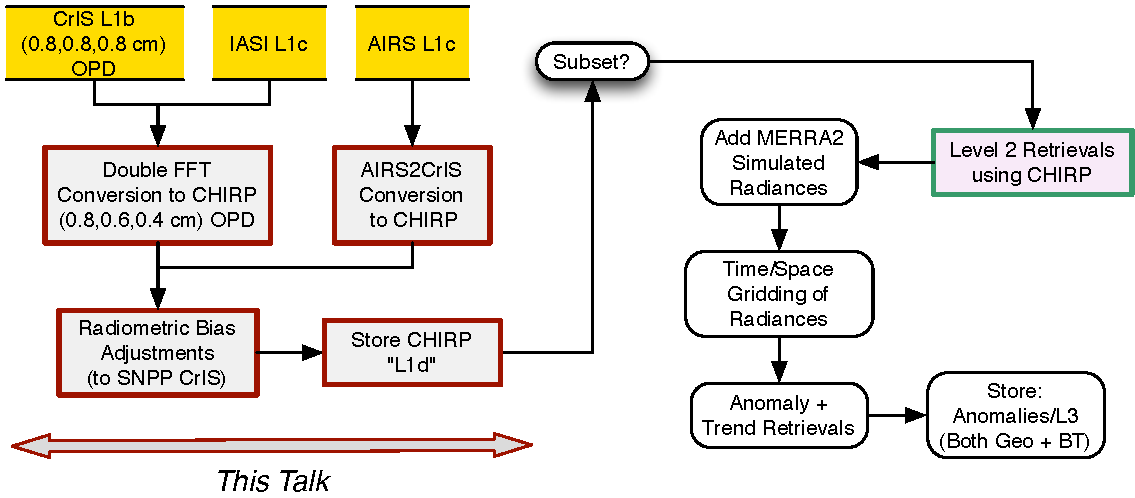
\includegraphics[width=1.0\linewidth]{./Figs/Pdf/airs2cris_stm_talk1_landscape.pdf}
\end{center}

\begin{block}{CHIRP: (Common or Climate) Hyperspectral InfraRed Product}
\begin{description}
\item[{OPD:}] 0.8 / 0.6 /0.4 cm
\item[{Spectral Spacing:}] 0.0625 / 0.0833 / 0.1250 \wn
\end{description}
\end{block}
\end{frame}

\begin{frame}[shrink=5,label={sec:org6b1374b}]{Why CHIRP}
\vspace{-0.2in}

\begin{itemize}
\item Convert AIRS, CrIS, IASI to a common spectral spectral response function
(SRF)
\item Correct for instrumental radiance offsets
\item Provides long-term radiance continuity over different instruments
\item Allows use of a single forward model (Radiative Transfer Algorithm) for
retrievals
\item Common SRF for AIRS/CrIS and IASI (1:30 and 9:30 equator crossings)
\item Applications
\begin{itemize}
\item Gridded (time/space) radiance products (“L1G”)
\item Geophysical retrievals (anomalies, trends) directly from all-sky radiance  anomaly/trends.  (See talk by L. Strow)
\end{itemize}
\item OLR trends directly from radiance trend retrievals (See talk by Sergio
DeSouza-Machado)
\item Use for Level 2 retrievals?  Only way to mitigate radiance calibration
difference among instruments and to achieve common sensitivity (both for
radiances and RTA)
\end{itemize}
\end{frame}






\begin{frame}[label={sec:orgf8c3420}]{CHIRP Data Flow}
\vspace{-0.1in}

\begin{center}
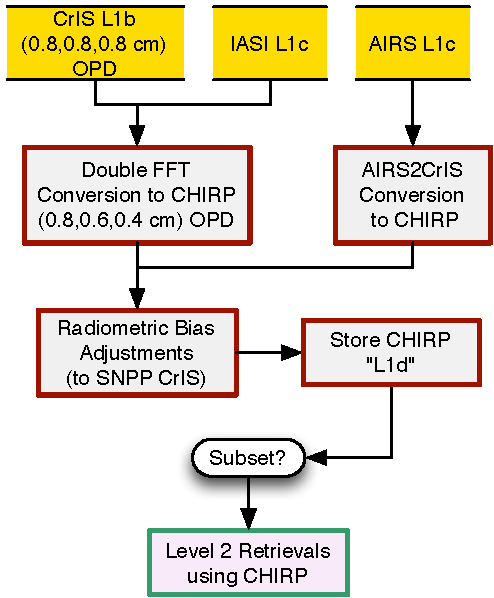
\includegraphics[width=0.6\linewidth]{./Figs/Pdf/airs2cris_stm_talk1_small.pdf}
\end{center}
\end{frame}


\begin{frame}[label={sec:org47a3590}]{AIRS, CrIS Differences}
\vspace{-0.1in}
\begin{itemize}
\item Instrument Line Shape (ILS): 
\begin{itemize}
\item CrIS: sinc
\item AIRS: 2378 ILS's, about 75\% in good shape
\end{itemize}
\item Footprints: roughly similar, some small issues
\item Orbits: sampling almost identical (later)
\item Noise: nominally similar
\item Calibration (later)
\end{itemize}

\begin{block}{ILS Differences}
\vspace{-0.05in}
\begin{itemize}
\item Large in B(T)
\item Existing approach: Retrievals use different forward models
\item \textcolor{maroon}{Cannot inter-calibrate AIRS and CrIS with different ILS functions!}
\item A hyperspectral radiance climatology requires same ILS between instruments
\end{itemize}

\large Our approach: Convert AIRS to the CrIS ILS
\end{block}
\end{frame}

\begin{frame}[label={sec:org4ed66b8}]{Spectral Differences Among AIRS, CrIS, IASI}
\begin{center}
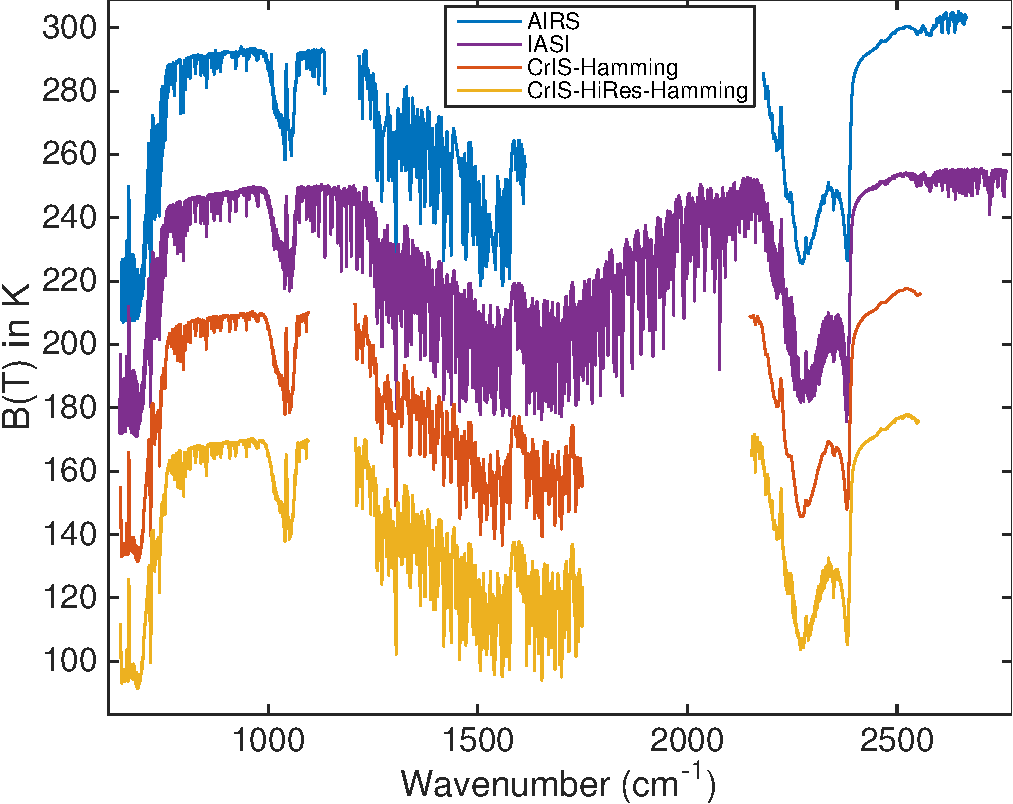
\includegraphics[width=0.85\linewidth]{./Figs/Pdf/hyperall_hamming.pdf}
\end{center}
\end{frame}

\begin{frame}[label={sec:orge1025ff}]{AIRS2CrIS Algorithm}
\vspace{-0.15in}
\begin{small}
\begin{itemize}
\item Simple deconvolution to 0.1 \wn grid
\item \(S_a r = r_A\), \(r_o = S_a^{-1} r_A\) using Moore-Penrose pseudoinverse
\item \(r_{A2C} = S_c \circledast r_o\)
\item Small additional terms using linear regression (mostly bias)
\item Errors below assume AIRS ILS functions are perfect
\end{itemize}
\end{small}
\vspace{-0.25in}
\begin{columns}
\begin{column}{0.55\columnwidth}
\begin{block}{\footnotesize AIRS2CrIS Mean Error (std. similar)}
\vspace{-0.1in}
\begin{center}
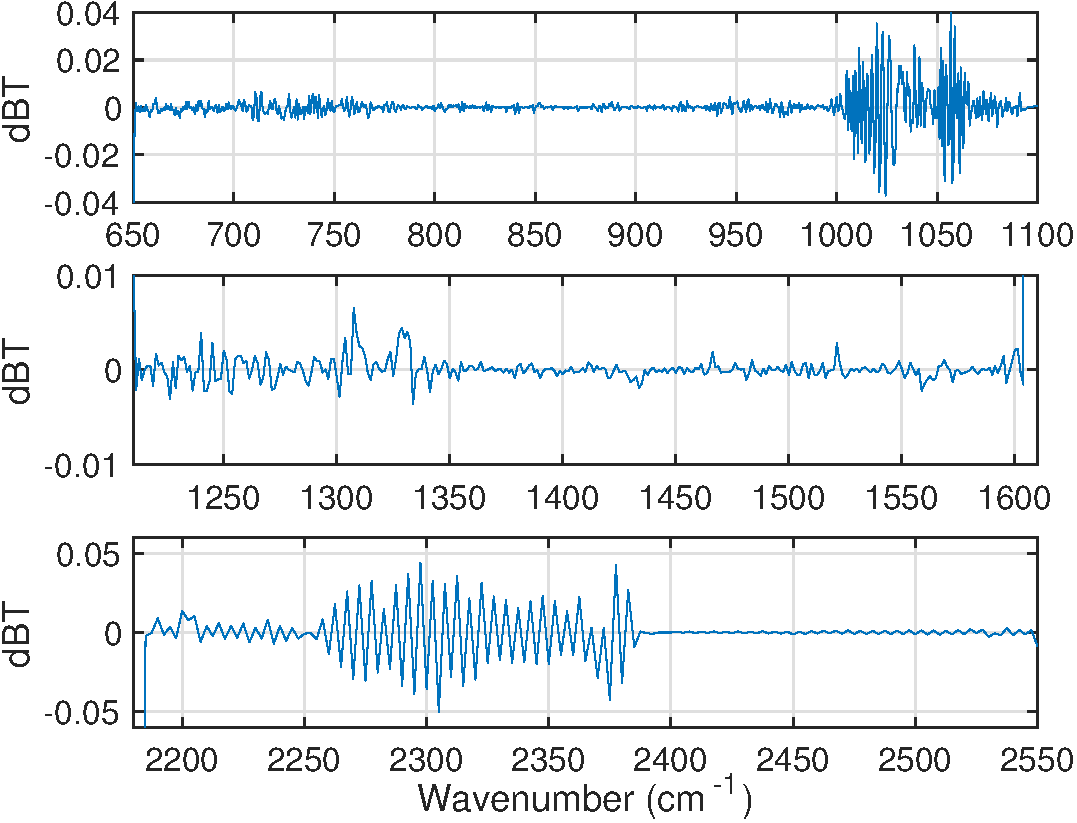
\includegraphics[width=0.95\linewidth]{./Figs/Pdf/ap_decon_corr.pdf}
\end{center}
\end{block}
\end{column}

\begin{column}{0.55\columnwidth}
\begin{block}{\footnotesize AIRS2CrIS Noise}
\vspace{-0.1in}
\begin{center}
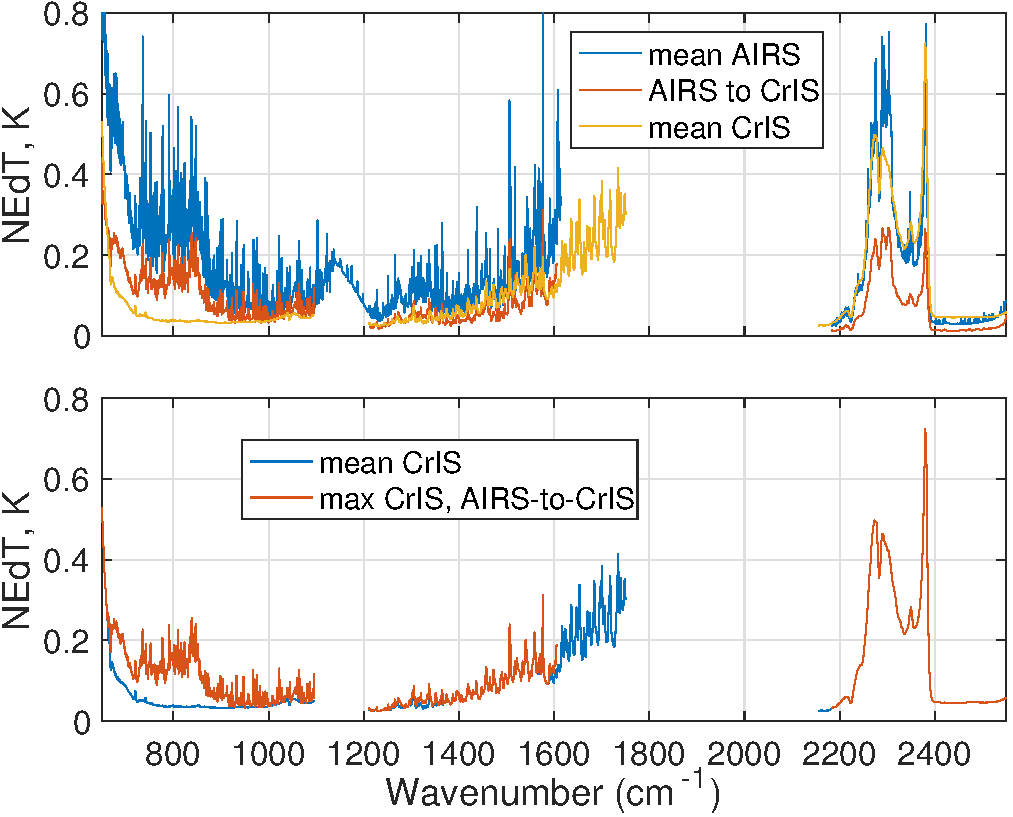
\includegraphics[width=0.95\linewidth]{./Figs/Pdf/a2cris_nedt.pdf}
\end{center}
\end{block}
\end{column}
\end{columns}

\vspace{-0.1in}
\small Shortwave sounding region max noise dominated by CrIS
\end{frame}

\begin{frame}[label={sec:orgeae713d}]{SNPP versus AIRS}
\vspace{-0.3in}

\begin{columns}
\begin{column}{0.55\columnwidth}
\begin{block}{\footnotesize 2016 SNOs}
\vspace{-0.1in}
\begin{center}
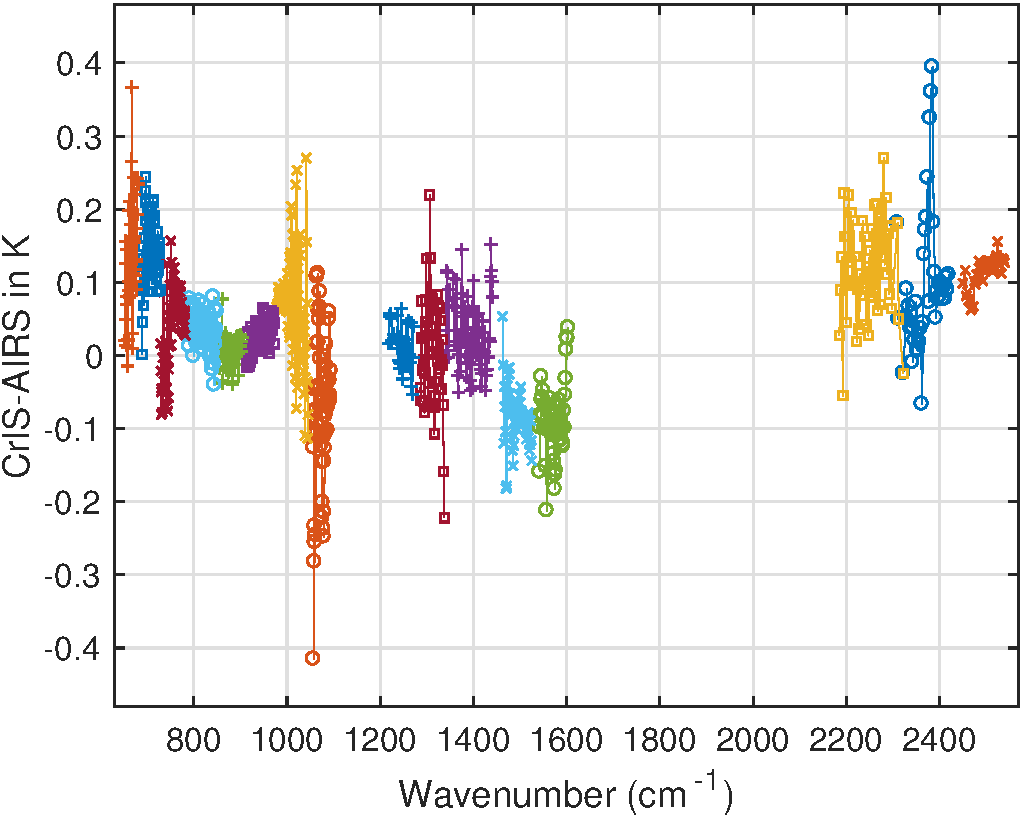
\includegraphics[width=\linewidth]{./Figs/Pdf/snpp_vs_airs_sno.pdf}
\end{center}
\end{block}
\end{column}

\begin{column}{0.55\columnwidth}
\begin{block}{\footnotesize 2016 Random Comparisons}
\vspace{-0.1in}
\begin{center}
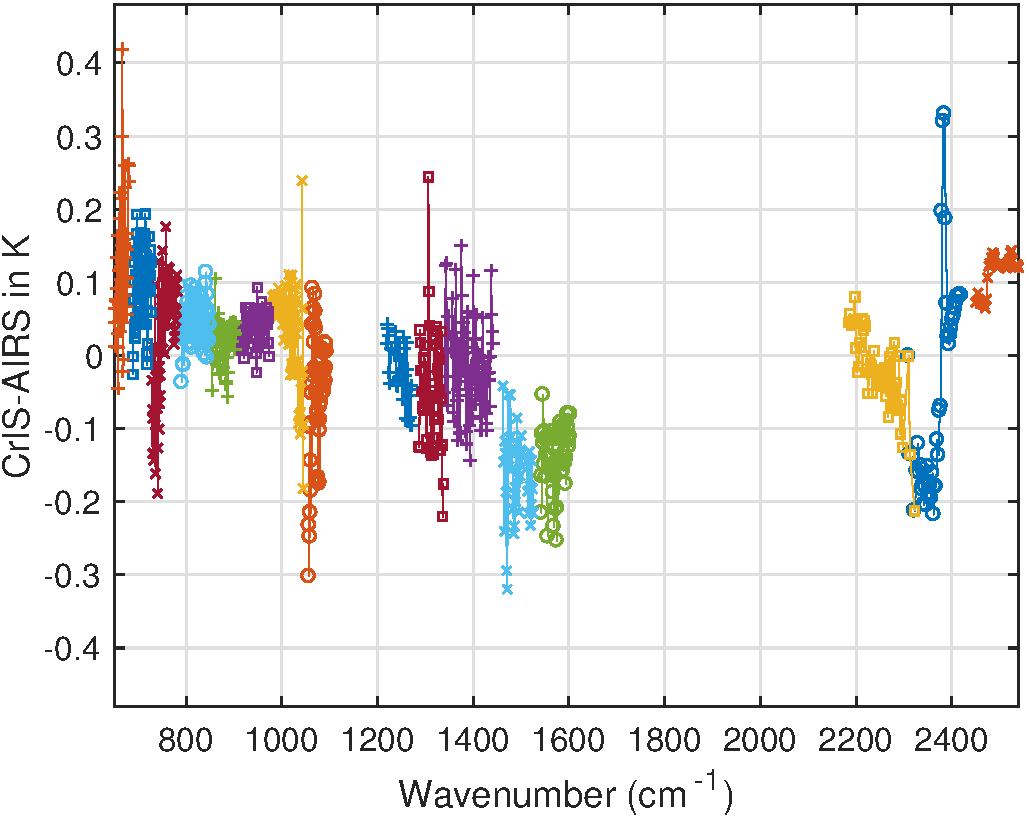
\includegraphics[width=\linewidth]{./Figs/Pdf/snpp_vs_airs_stats.pdf}
\end{center}
\end{block}
\end{column}
\end{columns}

\small
Sources for Differences
\vspace{-0.05in}
\begin{itemize}
\item Differential calibration AIRS modules
\item AIRS SRFs (widths and centroids)
\item Non-linearity: CrIS, AIRS?
\item etc.
\end{itemize}
\end{frame}

\begin{frame}[label={sec:orgc086e73}]{SNPP vs NOAA20 CrIS (via AIRS Snos)}
\vspace{-0.1in}

\begin{center}
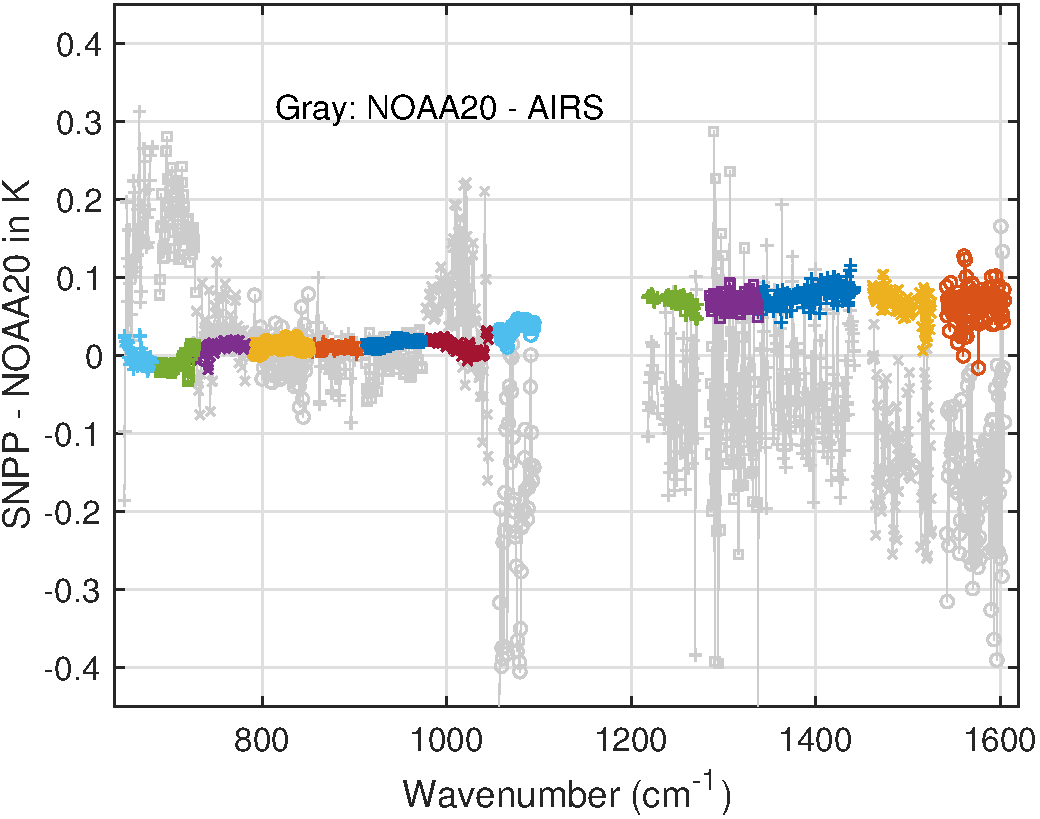
\includegraphics[width=0.65\linewidth]{./Figs/Pdf/sno_march2018_snpp_minus_noaa20_with_c2_airs_ingrey.pdf}
\end{center}

\vspace{-0.1in}

\small
\begin{itemize}
\item \emph{Preliminary}, NOAA20 CrIS non-linearity will be updated in July 2018
\item Connecting CrIS instruments together will be easier!
\item So far spatial, spectral, and sampling among CrIS instruments will be identical
\end{itemize}
\end{frame}
\end{document}